\subsection*{Problema 05}

\textbf{Enunciado:} Evaluar la integral definida 
mediante sumas de Riemann usando la partición 
regular del intervalo $[0, 1]$:
\begin{align*}
\int_{0}^{1} (x^3 - 1) \, dx
\end{align*}

\textbf{Solución:} 

Para evaluar la integral mediante la definición 
de límite de una suma de Riemann, utilizamos 
el extremo derecho del intervalo. Sea el 
intervalo $[a, b] = [0, 1]$ dividido en $n$ 
subintervalos de ancho igual a:
\begin{align*}
\Delta x = \dfrac{b - a}{n} = \dfrac{1 - 0}{n} = \dfrac{1}{n}
\end{align*}

Los puntos de la partición derecha son:
\begin{align*}
x_i = a + i \Delta x = 0 + i \left(\dfrac{1}{n}\right) = \dfrac{i}{n}
\end{align*}

Evaluamos la función $f(x) = x^3 - 1$ en 
cada punto $x_i$:
\begin{align*}
f(x_i) = \left(\dfrac{i}{n}\right)^3 - 1 
= \dfrac{i^3}{n^3} - 1
\end{align*}

Planteamos la suma de Riemann $S_n$:
\begin{align*}
S_n &= \sum_{i=1}^{n} f(x_i) \Delta x \\
S_n &= \sum_{i=1}^{n} \left(\dfrac{i^3}{n^3} - 1\right) \left(\dfrac{1}{n}\right)
\end{align*}

Distribuimos y aplicamos las propiedades 
de linealidad de las sumatorias:
\begin{align*}
S_n &= \dfrac{1}{n^4} \sum_{i=1}^{n} i^3 
- \dfrac{1}{n} \sum_{i=1}^{n} 1 \\
S_n &= \dfrac{1}{n^4} \sum_{i=1}^{n} i^3 - \dfrac{n}{n}
\end{align*}

Sustituimos la fórmula notable para 
la suma de cubos 
$\sum_{i=1}^{n} i^3 = \left[\dfrac{n(n+1)}{2}\right]^2$:
\begin{align*}
S_n &= \dfrac{1}{n^4} \left[\dfrac{n(n+1)}{2}\right]^2 - 1 \\
S_n &= \dfrac{1}{n^4} \left[\dfrac{n^2(n+1)^2}{4}\right] - 1
\end{align*}

Simplificamos la expresión algebraica:
\begin{align*}
S_n &= \dfrac{n^2(n+1)^2}{4n^4} - 1 \\
S_n &= \dfrac{(n+1)^2}{4n^2} - 1 \\
S_n &= \dfrac{1}{4} \left(\dfrac{n+1}{n}\right)^2 - 1 \\
S_n &= \dfrac{1}{4} \left(1 + \dfrac{1}{n}\right)^2 - 1
\end{align*}

Tomamos el límite cuando $n$ tiende a 
infinito para hallar el valor exacto 
de la integral definida:
\begin{align*}
\int_{0}^{1} (x^3 - 1) \, dx &= \lim_{n \to \infty} S_n \\
&= \lim_{n \to \infty} \left[ \dfrac{1}{4} \left(1 + \dfrac{1}{n}\right)^2 - 1 \right] \\
&= \dfrac{1}{4} (1 + 0)^2 - 1 \\
&= \dfrac{1}{4} - 1 = -\dfrac{3}{4}
\end{align*}

El valor de la integral definida es 
$-\dfrac{3}{4}$ o $-0.75$.

\begin{figure}[H]
	\centering
	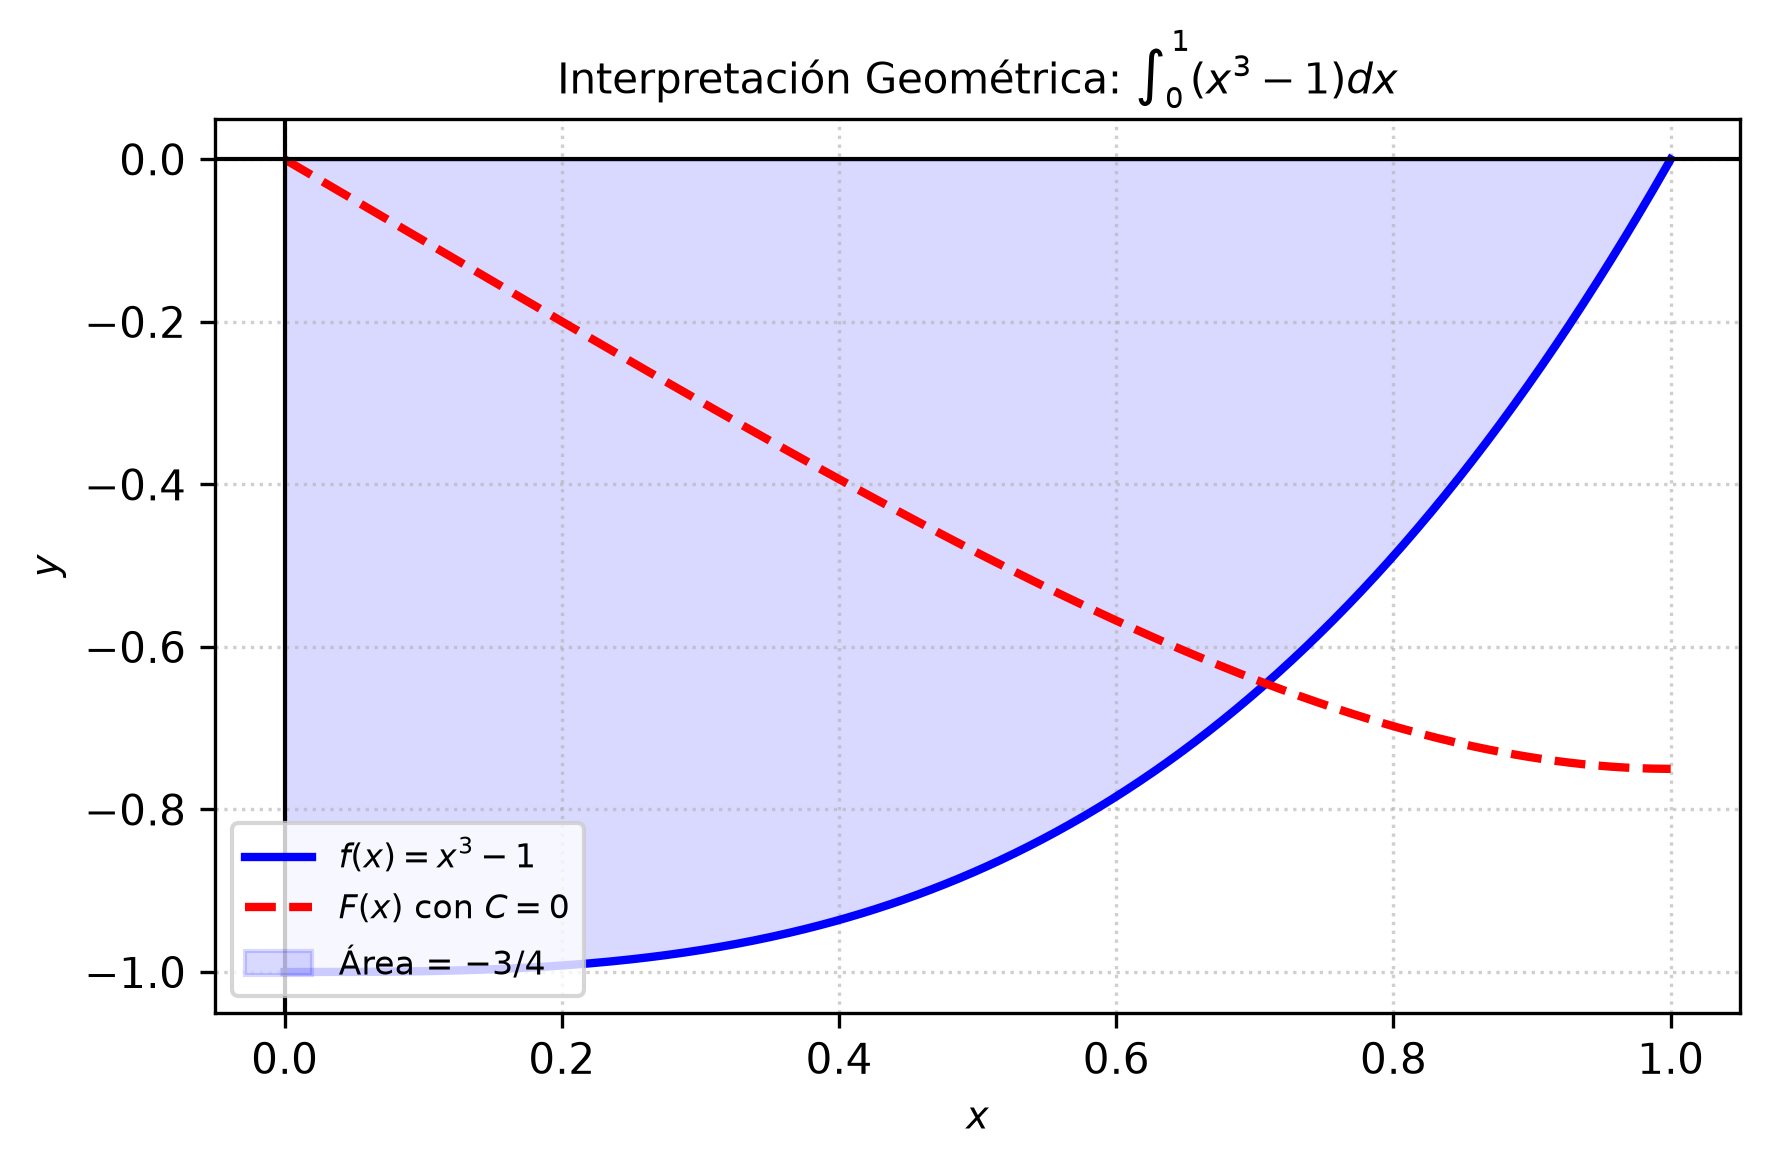
\includegraphics[width=\columnwidth]{semana_06/graficas/SEM06_P05_grafica.png}
	\caption{Representación gráfica de $f(x)$ y su antiderivada $F(x)$ evaluada para la constante de integración $C = 0$ (Problema 05).}
	\label{fig:problema05}
\end{figure}
